%%%%%%%%%%%%%%%%%%%%%%%%%%%%%%%%%%%%%%%%%
% Stylish Article
% LaTeX Template
% Version 2.1 (1/10/15)
%
% This template has been downloaded from:
% http://www.LaTeXTemplates.com
%
% Original author:
% Mathias Legrand (legrand.mathias@gmail.com) 
% With extensive modifications by:
% Vel (vel@latextemplates.com)
%
% License:
% CC BY-NC-SA 3.0 (http://creativecommons.org/licenses/by-nc-sa/3.0/)
%
%%%%%%%%%%%%%%%%%%%%%%%%%%%%%%%%%%%%%%%%%

%----------------------------------------------------------------------------------------
%	PACKAGES AND OTHER DOCUMENT CONFIGURATIONS
%----------------------------------------------------------------------------------------

\documentclass[10pt]{SelfArx} % Document font size and equations flushed left

\usepackage[english]{babel} % Specify a different language here - english by default

\usepackage{lipsum} % Required to insert dummy text. To be removed otherwise

%----------------------------------------------------------------------------------------
%	COLUMNS
%----------------------------------------------------------------------------------------


%\setlength{\columnsep}{0.55cm} % Distance between the two columns of text
\setlength{\fboxrule}{0.75pt} % Width of the border around the abstract

%----------------------------------------------------------------------
%   BOX OF 'ANALYSIS' PART, MODIFIED FROM THE 'COROLLARY' ENVIORMENT
%----------------------------------------------------------------------

\newcounter{dummy} 
\numberwithin{dummy}{section}
\newtheorem{corollaryT}[dummy]{Corollary}
\usepackage[framemethod=default]{mdframed} % Required for creating the theorem, definition, exercise and corollary boxes
% Corollary box
\newmdenv[skipabove=7pt,
skipbelow=7pt,
rightline=false,
leftline=true,
topline=false,
bottomline=false,
linecolor=gray,
backgroundcolor=black!5,
innerleftmargin=5pt,
innerrightmargin=5pt,
innertopmargin=5pt,
leftmargin=0.8cm,
rightmargin=0cm,
linewidth=4pt,
innerbottommargin=5pt]{cBox}
%\newenvironment{corollary}{\begin{cBox}\begin{corollaryT}}{\end{corollaryT}\end{cBox}}
\newenvironment{corollary}{\begin{cBox}\noindent{\bf\color{color1} 分析}}{\end{cBox}}





%----------------------------------------------------------------------------------------
%	COLORS
%----------------------------------------------------------------------------------------

\definecolor{color1}{RGB}{0,0,90} % Color of the article title and sections
\definecolor{color2}{RGB}{0,20,20} % Color of the boxes behind the abstract and headings

%----------------------------------------------------------------------------------------
%	HYPERLINKS
%----------------------------------------------------------------------------------------

\usepackage{hyperref} % Required for hyperlinks
\hypersetup{hidelinks,colorlinks,breaklinks=true,urlcolor=color2,citecolor=color1,linkcolor=color1,bookmarksopen=false,pdftitle={Title},pdfauthor={Author}}

%----------------------------------------------------------------------------------------
%	ARTICLE INFORMATION
%----------------------------------------------------------------------------------------

\JournalInfo{数学科学学院济梦数学基地"济梦之翼"项目组\\ 2018.11.17} % Journal information
%\Archive{Additional note} % Additional notes (e.g. copyright, DOI, review/research article)

\PaperTitle{高等数学(上)期中考试解答} % Article title

\Authors{笔记来源: 李少华\textsuperscript{1}, 记录: 杜黎\textsuperscript{2}, 整理: 彭任锋\textsuperscript{3}} % Authors
\affiliation{\textsuperscript{1}\textit{教授, 同济大学数学科学学院, 上海市杨浦区四平路1239号, 200092}} % Author affiliation
\affiliation{\textsuperscript{2}\textit{17级1班, 同济大学数学科学学院, 上海市杨浦区四平路1239号, 200092}} % Author affiliation
\affiliation{\textsuperscript{3}\textit{17级数理金融试验区, 同济大学数学科学学院, 上海市杨浦区四平路1239号, 200092}} % Author affiliation
%\affiliation{*\textbf{Corresponding author}: john@smith.com} % Corresponding author

\Keywords{高等数学, 微积分} % Keywords - if you don't want any simply remove all the text between the curly brackets
\newcommand{\keywordname}{关键词} % Defines the keywords heading name

%----------------------------------------------------------------------------------------
%	ABSTRACT
%----------------------------------------------------------------------------------------

\Abstract{本文由\LaTeX 排版, 由于工作量大, 时间紧迫, 所有题目均系笔者手算以及李少华老师笔记解出。本文件难免有疏漏或错误之处, 如有读者发现, 请不吝批评指正, 作者及负责人微信见附录。%\newline
}
%----------------------------------------------------------------------------------------

\begin{document}

\flushbottom % Makes all text pages the same height

\maketitle % Print the title and abstract box

\tableofcontents % Print the contents section

\thispagestyle{empty} % Removes page numbering from the first page

%----------------------------------------------------------------------------------------
%	ARTICLE CONTENTS
%----------------------------------------------------------------------------------------
% 正文从这里开始

%------------------------------------------------

\section{填空选择题}

\subsection{第一题}
若$\lim\limits_{x\to 0}(\displaystyle\frac{1-\sin x}{1+\sin 2x})^{\displaystyle\frac{1}{\tan kx}}=e$, 则$k=$\underline{\hbox to 20mm{}}
\begin{corollary}
	\begin{itemize}
		\item 想到重要极限$\lim\limits_{x\to 0}(1+x)^{\displaystyle\frac{1}{x}}=e$
		\item 取对数\qquad$\lim\limits_{x\to 0}\displaystyle\frac{\ln(x+1)}{x}=1$
		\item 注意在用L'Hospital法则时右边常数是不能一起求导的, 在这道题里面就是不要把$e$求掉了
	\end{itemize}
\end{corollary}
解: 原式两边取对数得
\begin{equation}
	1=\lim_{x\to 0}\displaystyle\frac{\ln\displaystyle\frac{1-\sin x}{1+\sin 2x}}{\tan kx}=\lim_{x\to 0}\displaystyle\frac{\displaystyle\frac{1-\sin x}{1+\sin 2x}-1}{kx}=\lim_{x\to 0}\displaystyle\frac{-\sin x-\sin 2x}{(1+\sin 2x)kx}=\lim_{x\to 0}\displaystyle\frac{-\displaystyle\frac{\sin x}{x}-\displaystyle\frac{\sin 2x}{x}}{k}=-\displaystyle\frac{3}{k}\nonumber
\end{equation}

故$k=-3$
\subsection{第二题}
设函数$f(x)=x^2, g(x)=x^3$, 则在区间$[0,2]$上, 由柯西中值定理确定的$\xi$为\underline{\hbox to 20mm{}}
\begin{corollary}
	\begin{itemize}
		\item 回想什么是柯西中值定理
	\end{itemize}
\end{corollary}
解: 由柯西中值定理, $\exists\xi\in(0,2)$, 使得
\begin{displaymath}
	\displaystyle\frac{f'(\xi)}{g'(\xi)}=\displaystyle\frac{f(2)-f(0)}{g(2)-g(0)}
\end{displaymath}

即
\begin{displaymath}
	\displaystyle\frac{2\xi}{3\xi^2}=\displaystyle\frac{4}{8}
\end{displaymath}

解得$\xi=\displaystyle\frac{4}{3}$

\subsection{第三题}
设$f(x)=x^{2^x}$, 则d$f(x)=$\underline{\hbox to 20mm{}}
\begin{corollary}
	\begin{itemize}
		\item 直接复合函数求导是不好做的, 我们可以考虑取对数\qquad$\ln f=2^x\ln x$
	\end{itemize}
\end{corollary}
解: 原式两边取对数得
\begin{displaymath}
	\ln f=2^x\ln x
\end{displaymath}

两边求微分得
\begin{displaymath}
	\displaystyle\frac{{\rm d}f}{f}=(\displaystyle\frac{2^x}{x}+2^x\ln 2x){\rm d}x
\end{displaymath}

故
\begin{displaymath}
	{\rm df}=f(\displaystyle\frac{2^x}{x}+2^x\ln 2x){\rm d}x=x^{2^x}(\displaystyle\frac{2^x}{x}+2^x\ln 2x){\rm d}x
\end{displaymath}
\subsection{第四题}
曲线$y=x^2$上与$x+2y-2=0$平行的切线方程为\underline{\hbox to 20mm{}}
\begin{corollary}
	\begin{itemize}
		\item 切线方程主要是找切点, 一般的做法是设出切点然后解出来
	\end{itemize}
\end{corollary}
解: 设切点为$(x_0,x_0^2)$, 则相应的切线方程为$y-x_0^2=2x_0(x-x_0)$, 由题意知斜率为$-\displaystyle\frac{1}{2}$, 即$x_0=-\displaystyle\frac{1}{4}$, 故切线方程为$y-\displaystyle\frac{1}{16}=-\displaystyle\frac{1}{2}(x+\displaystyle\frac{1}{4})$, 即$y=-\displaystyle\frac{1}{2}x-\displaystyle\frac{1}{16}$
\subsection{第五题}
已知$f(x)=\displaystyle\frac{e^x-b}{(x-a)(x-b)}$, 且$x=e$为$f(x)$的无穷间断点, $x=1$为$f(x)$的可去间断点, 则$b=$\underline{\hbox to 20mm{}}
\begin{corollary}
	\begin{itemize}
		\item 回忆无穷间断点和可去间断点的定义, 这道题先从可去间断点入手, $x=1$为可去间断点说明$f(x)$在$x=1$处不连续但是$\lim\limits_{x\to 1}f(x)$存在, 即此时$f(x)$为$\displaystyle\frac{0}{0}$未定型式
	\end{itemize}
\end{corollary}
解: 由于$x=1$为可去间断点, 故$\begin{cases}
e-b=0\\
(1-a)(1-b)=0
\end{cases}$, 解得$a=1,b=e$, 验证可知$x=e$的确是无穷间断点
\subsection{第六题}
设$f(x)=\displaystyle\frac{(x-1)(x-2)\cdots(x-n)}{(x+1)(x+2)\cdots(x+n)}$, 则$f'(1)=$\underline{\hbox to 20mm{}}
\begin{corollary}
	\begin{itemize}
		\item 求解导数, 可以直接求导, 也可以用到极限定义。 这道题形式复杂, 如果直接求导实在是太麻烦, 可以考虑用极限定义, 当然直接法也是可以做的。
		\item 考场上如果不大确定自己的答案, 可以验证简单的情况, 比如$n=1$
	\end{itemize}
\end{corollary}
解:(直接求导法)  设分母为$g(x)$, 分子为$h(x)$, 则$f'(x)=\displaystyle\frac{h'(x)g(x)-g'(x)h(x)}{g^2(x)}$, 注意到$h(1)=0$, $h'(1)=(-2)(-3)\cdots(-(n-1))$, 故$f'(1)=\displaystyle\frac{h'(1)g(1)}{g^2(1)}=\displaystyle\frac{(-1)^{n-1}(n-1)!}{(n+1)!}=\displaystyle\frac{(-1)^{n-1}}{n(n+1)}$

\indent

\noindent 解:(极限法) 由导数的定义
\begin{displaymath}
	f'(1)=\lim_{x\to 1}\displaystyle\frac{f(x)-f(1)}{x-1}=\lim_{x\to 1}\displaystyle\frac{(x-2)(x-3)\cdots(x-n)}{(x+1)(x+2)\cdots(x+n)}==\displaystyle\frac{(-1)^{n-1}(n-1)!}{(n+1)!}=\displaystyle\frac{(-1)^{n-1}}{n(n+1)}
\end{displaymath} 
\subsection{第七题}
设当$x\to 1$时, $1-\displaystyle\frac{m}{1+x+\cdots+x^{m-1}}$是$x-1$的等价无穷小, 则$m=$\underline{\hbox to 20mm{}}
\begin{corollary}
	\begin{itemize}
		\item 回忆等价无穷小的定义, 按照定义来做即可
		\item 熟悉公式$x^m-1=(x-1)(1+x+\cdots+x^{m-1})$
	\end{itemize}
\end{corollary}
解: 由已知得
\begin{displaymath}
	1=\lim_{x\to 1}\displaystyle\frac{1-\displaystyle\frac{m}{1+x+\cdots+x^{m-1}}}{x-1}=\lim_{x\to 1}\displaystyle\frac{1+x+\cdots+x^{m-1}-m}{x^m-1}\xlongequal{\text{L'Hospital}}\lim_{x\to 1}\displaystyle\frac{1+2x+\cdots+(m-1)x^{m-2}}{mx^{m-1}}\xlongequal{\text{直接代入}}\displaystyle\frac{m-1}{2}
\end{displaymath}

故$m=3$
\subsection{第八题}
设当$x\to 0$时, 下列无穷小
\begin{center}
	\textcircled{1} $\sqrt{1+\tan x}-\sqrt{1+\sin x}$\qquad\textcircled{2} $\sqrt{1+2x}-\sqrt[3]{1+3x}$
	
	\textcircled{3} $x(\arcsin x-x)$\qquad\qquad\textcircled{4} $e^{x^4-x}-1$
\end{center}

中, 从低阶到高阶的排列顺序为\underline{\hbox to 20mm{}}

A. \textcircled{1}\textcircled{2}\textcircled{3}\textcircled{4}
B. \textcircled{3}\textcircled{1}\textcircled{2}\textcircled{4}
C. \textcircled{4}\textcircled{3}\textcircled{2}\textcircled{1}
D. \textcircled{4}\textcircled{2}\textcircled{1}\textcircled{3}
\begin{corollary}
	\begin{itemize}
		\item 想到等价无穷小以及Taylor公式
		\item 分析阶数就不用管常数部分了
		\item 相减不能直接等价无穷小, 考虑Taylor公式
		\item 如果在考试里面, 观察选项的特点, 你可以节省时间只要算前三个就可以确定答案了
	\end{itemize}
\end{corollary}
解: 我们逐一讨论每一个无穷小的阶
\begin{enumerate}
	\item[\textcircled{1}] 分子有理化
		\begin{displaymath}
			\sqrt{1+\tan x}-\sqrt{1+\sin x}=\displaystyle\frac{\tan x-\sin x}{\sqrt{1+\tan x}+\sqrt{1+\sin x}}\propto\tan x(1-\cos x)\sim x\cdot x^2=x^3
		\end{displaymath}
	\item[\textcircled{2}] 应用Taylor展开
		\begin{displaymath}
			\sqrt{1+2x}-\sqrt[3]{1+3x}=(1+x-\displaystyle\frac{x^2}{2}+o(x^2))-(1+x-x^2+o(x^2))\sim x^2
		\end{displaymath}
	\item[\textcircled{3}] 令x=sin t, 则$x\to 0$时$t\to 0$
		\begin{displaymath}
			x(\arcsin x-x)=\sin t(t-\sin t)\sim t\cdot t^3=t^4\sim x^4
		\end{displaymath}
	\item[\textcircled{4}] 直接Taylor展开(事实上起作用的是$-x$, 你可以忽略$x^4$的影响)
		\begin{displaymath}
			e^{x^4-x}-1=1+(x^4-x)+o(x)-1\sim x
		\end{displaymath}
\end{enumerate}

\section[计算题]{计算题(每小题6分)}
\subsection{第一题}
求极限$\lim\limits_{x\to 0}\displaystyle\frac{1}{x^3}[(\displaystyle\frac{2+\cos x}{3})^x -1]$
\begin{corollary}
	\begin{itemize}
		\item 幂指函数不好求导, 可以变为对数恒等式
	\end{itemize}
\end{corollary}
解: 由已知得
\begin{displaymath}
	(\displaystyle\frac{2+\cos x}{3})^x -1=e^{x\ln(\displaystyle\frac{2+\cos x}{3})}-1\sim x\ln\displaystyle\frac{2+\cos x}{3}\sim x\cdot\displaystyle\frac{\cos x-1}{3}\sim x\cdot (-\displaystyle\frac{x^2}{2})=-\displaystyle\frac{x^3}{2}
\end{displaymath}

故原式$=-\displaystyle\frac{1}{2}$
\subsection{第二题}
设函数$y=y(x)$由参数方程$\begin{cases}
x=t+e^t\\
y=\sin t
\end{cases}$确定, 求$\displaystyle\frac{{\rm d}^2 y}{{\rm d} x^2}$
\begin{corollary}
	\begin{itemize}
		\item 本题考查参数方程求导, 一定要注意$\displaystyle\frac{{\rm d}^2y}{{\rm d}x^2}\neq \displaystyle\frac{{\rm d}^2y}{{\rm d}t^2}\cdot\displaystyle\frac{{\rm d}t^2}{{\rm d}^2x}$, 正确的公式是
		\begin{displaymath}
			\displaystyle\frac{{\rm d}^2y}{{\rm d}x^2}=\displaystyle\frac{\dot{x}\ddot{y}-\dot{y}\ddot{x}}{\dot{x}^3}
		\end{displaymath}
		
		这里$\dot{x},\ddot{x}$为$x$对$t$的一阶、二阶导数, $\dot{y},\ddot{y}$的一阶、二阶导数
	\end{itemize}
\end{corollary}
解: 由已知得
\begin{displaymath}
	\displaystyle\frac{{\rm d}x}{{\rm d}t}=1+e^t\qquad\displaystyle\frac{{\rm d}y}{{\rm d}t}=\cos t
\end{displaymath}

故一阶导为
\begin{displaymath}
	\displaystyle\frac{{\rm d}y}{{\rm d}x}=\displaystyle\frac{\cos t}{1+e^t}
\end{displaymath}

对上式微分
\begin{displaymath}
{\rm d}\displaystyle\frac{{\rm d}y}{{\rm d}x}={\rm d}\displaystyle\frac{\cos t}{1+e^t}=\displaystyle\frac{-\sin t(1+e^t)-e^t\cos t}{(1+e^t)^2}{\rm d}t=\displaystyle\frac{-\sin t(1+e^t)-e^t\cos t}{(1+e^t)^3 }{\rm d}x
\end{displaymath}

故
\begin{displaymath}
\displaystyle\frac{{\rm d}^2y}{{\rm d}x^2}=\displaystyle\frac{-\sin t(1+e^t)-e^t\cos t}{(1+e^t)^3 }
\end{displaymath}
\subsection{第三题}
求函数$y=\displaystyle\frac{2x-1}{x^2+3x-4}$的$n$阶导数
\begin{corollary}
	\begin{itemize}
		\item 待定系数法设$\displaystyle\frac{cx+d}{(x-a)(x-b)}=\displaystyle\frac{A}{x-a}+\displaystyle\frac{B}{x-b}$, 解出$A,B$, 事实上这在你们学习积分的时候也很常用, 也有拓展形式
		\begin{displaymath}
			\displaystyle\frac{P(x)}{(x-a)^n(x-b)^m}=\displaystyle\frac{A_1}{x-a}+\displaystyle\frac{A_2}{(x-a)^2}+\cdots+\displaystyle\frac{A_n}{(x-a)^n}+\displaystyle\frac{B_1}{x-b}+\displaystyle\frac{B_2}{(x-b)^2}+\cdots+\displaystyle\frac{B_m}{(x-b)^m}
		\end{displaymath}
		\item 直接用Leibniz公式, 但是会有些麻烦
	\end{itemize}
\end{corollary}
解: 由已知得
\begin{displaymath}
	y=\displaystyle\frac{2x-1}{x^2+3x-4}=\displaystyle\frac{1/5}{x-1}+\displaystyle\frac{9/5}{x+4}
\end{displaymath}

则
\begin{displaymath}
y^{(n)}=\displaystyle\frac{(-1)^nn!}{5(x-1)^{n+1}}+\displaystyle\frac{(-1)^n\cdot 9n!}{5(x+4)^{n+1}}
\end{displaymath}
\section[计算题]{计算题(每小题8分)}
\subsection{第一题}
求曲线$y=\displaystyle\frac{x^3}{1-x^2}+\arctan(2+x)$的渐近线方程
\begin{corollary}
	\begin{itemize}
		\item 先考虑垂直渐近线
		\item 回忆渐近线的求法$\begin{cases}
		k=\lim\limits_{x\to\infty}\displaystyle\frac{y}{x}\\
		b=\lim\limits_{x\to\infty}y-kx
		\end{cases}$
	\end{itemize}
\end{corollary}
解: 垂直渐近线$x=\pm 1$

再求解其他渐近线
\begin{gather}
	k=\lim_{x\to\infty}\displaystyle\frac{y}{x}=-1\nonumber\\
	b_1=\lim_{x\to+\infty}y-kx=\displaystyle\frac{\pi}{2}\nonumber\\
	b_2=\lim_{x\to-\infty}y-kx=-\displaystyle\frac{\pi}{2}\nonumber
\end{gather}

故我们所求的渐近线为$x=\pm 1$, $y=-x\pm\displaystyle\frac{\pi}{2}$
\subsection{第二题}
求极限$\lim\limits_{x\to 0}\displaystyle\frac{\cos x-e^{-\displaystyle\frac{x^2}{2}}}{\ln(1+2x^2)(2^{x^2}-1)}$
\begin{corollary}
	\begin{itemize}
		\item 分子Taylor展开, 注意Taylor一定要展开到不为0的项
		\item 分母可以等价代换
	\end{itemize}
\end{corollary}
解: 先分析分子, $x\to 0$时
\begin{displaymath}
	\cos x-e^{-\displaystyle\frac{x^2}{2}}=1-\displaystyle\frac{x^2}{2}+\displaystyle\frac{x^4}{4}+o(x^4)-(1-\displaystyle\frac{x^2}{2}+\displaystyle\frac{x^4}{8}+o(x^4))=\displaystyle\frac{x^4}{8}+o(x^4)
\end{displaymath}

再分析分母
\begin{displaymath}
	\ln(1+2x^2)(2^{x^2}-1)\sim 2x^2(2^{x^2}-1)
\end{displaymath}

故
\begin{displaymath}
	\lim_{x\to 0}\displaystyle\frac{\cos x-e^{-\displaystyle\frac{x^2}{2}}}{\ln(1+2x^2)(2^{x^2}-1)}=\lim_{x\to 0}\displaystyle\frac{\displaystyle\frac{1}{8}x^4}{2x^2(2^{x^2}-1)}=\lim_{x\to 0}\displaystyle\frac{x^2}{16(2^{x^2}-1)}\xlongequal{L'Hospital}\lim_{x\to 0}\displaystyle\frac{2x}{16\cdot 2^{x^2}\cdot 2x\ln 2}=\displaystyle\frac{1}{16\ln 2}
\end{displaymath}
\subsection{第三题}
设$y=y(x)$由$\arctan\displaystyle\frac{y}{x}=\ln\sqrt{x^2+y^2}$确定, 求$\displaystyle\frac{{\rm d}^2 y}{{\rm d} x^2}$
\begin{corollary}
	\begin{itemize}
		\item 隐函数求导
	\end{itemize}
\end{corollary}
解: 等式两边微分, 得
\begin{displaymath}
	\displaystyle\frac{1}{1+(\displaystyle\frac{y}{x})^2}\displaystyle\frac{x{\rm d}y-y{\rm d}x}{x^2}=\displaystyle\frac{x{\rm d}x+y{\rm d}y}{x^2+y^2}
\end{displaymath}

即
\begin{displaymath}
	\displaystyle\frac{{\rm d}y}{{\rm d}x}=\displaystyle\frac{x+y}{x-y}
\end{displaymath}

故
\begin{displaymath}
{\rm d}\displaystyle\frac{{\rm d}y}{{\rm d}x}=\displaystyle\frac{({\rm d}x+{\rm d}y)(x-y)-(x+y)({\rm d}x-{\rm d}y)}{(x-y)^2}=\displaystyle\frac{-2y{\rm d}x+2x{\rm d}y}{(x-y)^2}=\displaystyle\frac{-2y+2x\cdot\displaystyle\frac{x+y}{x-y}}{(x-y)^2}{\rm d}x=\displaystyle\frac{2x^2+2y^2}{(x-y)^3}{\rm d}x
\end{displaymath}

故
\begin{displaymath}
	\displaystyle\frac{{\rm d}^2 y}{{\rm d} x^2}=\displaystyle\frac{2x^2+2y^2}{(x-y)^3}
\end{displaymath}
\subsection{第四题}
求曲线$y=\ln x$的最大曲率
\begin{corollary}
	\begin{itemize}
		\item 曲率公式$\kappa=\displaystyle\frac{|y''|}{(1+y'^2)^{\displaystyle\frac{3}{2}}}$
	\end{itemize}
\end{corollary}
解: 直接套用公式得
\begin{displaymath}
	\kappa=\displaystyle\frac{|y''|}{(1+y'^2)^{\displaystyle\frac{3}{2}}}=\sqrt{\displaystyle\frac{x^2}{(1+x)^3}}
\end{displaymath}

令$x+1=\displaystyle\frac{1}{t}$以及$g(t)=t^3-2t^2+t$, $t\in (0,\displaystyle\frac{1}{2})$, 则$g'(t)=3t^2-4t+1=(3t-1)(t-1)$

当$0<t<\displaystyle\frac{1}{3}$时, $g'(t)>0$, 当$\displaystyle\frac{1}{3}<t<\displaystyle\frac{1}{2}$时, $g'(t)<0$

故当$t=\displaystyle\frac{1}{3}$时, $g(t)$取得最大值$\displaystyle\frac{4}{27}$, 即$\kappa_{max}=\displaystyle\frac{4}{27}$
\section[解答题]{解答题(本题10分)}
求函数$f(x)=\displaystyle\frac{1}{1+|x|}+\displaystyle\frac{1}{1+|x-2|}$的单调区间
\begin{corollary}
	\begin{itemize}
		\item 分区间进行讨论
	\end{itemize}
\end{corollary}
解: 分情况讨论
\begin{enumerate}
	\item $x\geqslant 2$时, $f(x)=\displaystyle\frac{1}{1+x}+\displaystyle\frac{1}{x-1}$, 显然$f(x)$在$[2,+\infty)$上单调递减
	\item $0\leqslant x<2$时, $f(x)=\displaystyle\frac{1}{1+x}+\displaystyle\frac{1}{3-x}$, $f'(x)=-\displaystyle\frac{1}{(1+x)^2}+\displaystyle\frac{1}{(3-x)^2}=\displaystyle\frac{4(2x-2)}{(x+1)^2(x-3)^2}$
	
	故$f(x)$在$[0,1]$上单调递减, 在$(1,2)$上单调递增
	\item $x<0$时, $f(x)=\displaystyle\frac{1}{1-x}+\displaystyle\frac{1}{3-x}$, $f'(x)>0$, 故$f(x)$在$[-2,0)$上单调递增
\end{enumerate}

综上, $f(x)$在$(-\infty,0),(1,2)$上单调递增, 在$[0,1],[2,+\infty)$上单调递减
\section[解答题]{解答题(本题10分)}
证明方程$2^x=x^2+1$仅有三个根
\begin{corollary}
	\begin{itemize}
		\item 先看看有没有显而易见的零点
		\item 肯定是构造函数, 根据单调性, 介值定理来分析零点
		\item 直接构造, $f'(x)=0$还是超越方程, 不好求解, 有没有别的构造方法?
	\end{itemize}
\end{corollary}
Pf: 构造$f(x):=\displaystyle\frac{x^2+1}{2^x}-1$, 则
\begin{displaymath}
	f'(x)=\displaystyle\frac{-x^2+\displaystyle\frac{2}{\ln 2}x-1}{2^x}
\end{displaymath}

$\Delta=\displaystyle\frac{4}{\ln^2 2}-4>0$, 故$\exists x_1,x_2$, 使得$f(x_1)=f(x_2)=0$, 由于$f'(0)<0, f'(1)>0, f'(2)>0, f'(3)<0$, 故$0<x_1<1, 2<x_2<3$, 故$f(x)$在$[3,+\infty)$上单调递减, 又$f(3)>0,f(10)<0$, 故$\exists x_0\in(3,10)$, 使得$f(x_0)=0$, 又$f(0)=f(1)=0$, 故原方程有三个根, Q.E.D.
\begin{figure}[h]
	\centering
	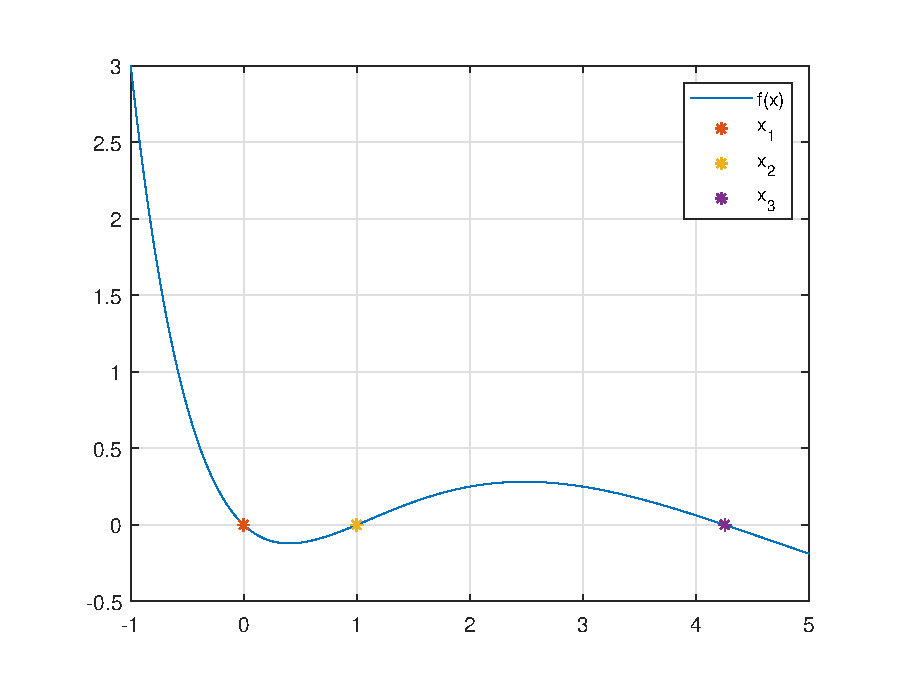
\includegraphics[width=0.5\textwidth]{1}
	\caption{根的分布图像}
\end{figure}


\section[解答题]{解答题(本题6分)}
设$f(x)$在$(-\infty,+\infty)$上有连续的三阶导数, 证明: 存在实数$\xi\in(-1,1)$, 使得
\begin{displaymath}
	\displaystyle\frac{f'''(\xi)}{6}=\displaystyle\frac{f(1)-f(-1)}{2}-f'(0)
\end{displaymath}
\begin{corollary}
	\begin{itemize}
		\item 高阶导数, 想到带Lagrange余项的Taylor展开, 在哪一点展开?
		\item 展开以后两个3阶导数, 怎么办?
	\end{itemize}
\end{corollary}
Pf: 将$f(x)$在$x=0$处Taylor展开, 并分别代入$1,-1$得
\begin{gather}
	f(1)=f(0)+f'(0)+\displaystyle\frac{f''(0)}{2}+\displaystyle\frac{f'''(\xi_1)}{6}\nonumber\\
	f(-1)=f(0)-f'(0)+\displaystyle\frac{f''(0)}{2}-\displaystyle\frac{f'''(\xi_2)}{6}\nonumber
\end{gather}

两式相减得
\begin{displaymath}
	\displaystyle\frac{f(1)-f(-1)}{2}=f'(0)+\displaystyle\frac{1}{12}(f'''(\xi_1)+f'''(\xi_2))
\end{displaymath}

由于$f'''(x)$连续, 故可由介值定理, 对于$\displaystyle\frac{f'''(\xi_1)+f'''(\xi_2)}{2}$, $\displaystyle\frac{f'''(\xi_1)+f'''(\xi_2)}{2}$的值是介于$f'''(\xi_1)$和$f'''(\xi_2)$的, 因此$\exists\xi\in(\xi_2,\xi_1)$, 使得$f'''(\xi)=\displaystyle\frac{f'''(\xi_1)+f'''(\xi_2)}{2}$, 代回上式, 则
\begin{displaymath}
	\displaystyle\frac{f'''(\xi)}{6}=\displaystyle\frac{f(1)-f(-1)}{2}-f'(0)
\end{displaymath}

Q.E.D.
%------------------------------------------------
% 感谢啥的乱七八糟的东西
\phantomsection
\section{Summary}
\subsection{关于卷子}
这应该是各位大一萌新们来到同济大学的第一次考试, 一般大一上的考试老师都会出得稍微难一些, 目的在于告诉你大学是没那么好读的, 要认真努力才好。总体而言这张卷子难度适中, 应该是具有一定区分度的, 考查的点也很多, 很细, 如果没有扎实的基本功, 笔者认为你是很难在有限的时间里面做完的。
\subsection{关于L'Hospital法则}
微信群里传了这么张图片
\begin{figure}[h]
	\centering
	\includegraphics[width=0.4\textwidth]{IMG_7085.jpg}
\end{figure}

关于L'Hospital法则, 确实很容易理解, 也确实很容易操作(求导谁不会呢), 但是使用的时候还是要考虑以下问题
\begin{itemize}
	\item 能不能用? 也就是说是否是$\displaystyle\frac{0}{0}$或$\displaystyle\frac{\infty}{\infty}$未定形式
	\item 如果L'Hospital求出极限不存在, 是不能说明原极限不存在的
	
	e.g. $\lim\limits_{x\to \infty}\displaystyle\frac{x+\sin x}{x}=1$, 但是L'Hospital后$\lim\limits_{x\to\infty}1+\cos x$不存在
	\item L'Hospital一般用于函数形式简单的情形, 否则有些题目你傻乎乎的洛一年都洛不出结果来
	\item 还有, 边洛边观察, 是否可以等价无穷小替换? 是否可以Taylor公式?
\end{itemize}

笔者在自己数学老师的影响下, 对极限问题还是有一定研究的。笔者认为, 极限形式上的化简, 以及Taylor公式是更重要的, 但是用Taylor一定要展开的"足够充分", 而且最好不要省去无穷小量, 除非你很有把握。
\subsection{关于未来的学习}
笔者认为, 到了大学, 一样的不要放松了, 特别是高等数学, 毕竟5学分是很影响GPA的。高数要注重平时的学习, 注重概念的理解, 比如我在上面写的L'Hospital的注意事项, 你在学习的时候有注意到嘛? 我希望你有。题可以刷, 但是不要只刷题了, 这不是高中, 老师还会给你一轮二轮三轮复习的, 刷题要有总结, 有琢磨, 就像这篇PDF一样。

此外, 多和你的高数老师交流, 如果你有困惑, 我觉得你找他们是非常有效的。
\section*{Acknowledgments} % The \section*{} command stops section numbering

\addcontentsline{toc}{section}{Acknowledgments} % Adds this section to the table of contents

感谢李少华教授, 张世瑞同学以及数学科学学院济梦数学基地"济梦之翼"项目组的支持。
\section*{附录}
\addcontentsline{toc}{section}{附录}
\begin{figure}[h]
	\centering
	\subfigure[负责人: 小济]{\includegraphics[width=0.3\textwidth]{IMG_0260.jpg}}
	\subfigure[整理人: 彭任锋]{\includegraphics[width=0.3\textwidth]{IMG_0261.jpg}}
\end{figure}

%----------------------------------------------------------------------------------------
%	REFERENCE LIST
%----------------------------------------------------------------------------------------
\phantomsection
\bibliographystyle{unsrt}
%\bibliography{sample}

%----------------------------------------------------------------------------------------

\end{document}